\noindent
{\bf Collaborative Research: Mathematical modeling and simulation of
self-assembling amphiphilic particles in solvent} \\
%{\bf {Collaborative Research: Mathematical modeling and coarse-grained simulations of self-assembly of amphiphilic Janus particles in a solvent}}\\
{\em Rolf Ryham (lead PI, Fordham University), Bryan Quaife (PI,
Florida State University), and Yuan-Nan Young (PI, New Jersey Institute of Technology)}
\section{Background}
\label{sec:background}
The goal of this collaborative proposal is to use mathematical modeling
and numerical simulations to investigate the dynamic self-assembly of
amphiphilic particles interacting via hydrophobic forces
in solvent. Amphiphilic particles (such as lipid molecules) possess
both hydrophobic and hydrophilic structures. In a viscous solvent they
self-assemble into meso-/macroscopic structures (such as micelles and
bilayers of lipids) to shield their hydrophobic parts from contact with
the solvent (water) molecules.
%
%\subsection{Hydrophobic Forces}
%\label{sec:hydrophobicforce}
%
Such self-assembly of amphiphiles via hydrophobic forces is ubiquitous in biology and biophysics \cite{Israelachvili1954},
%The hydrophobic force is a ubiquitous molecular interaction in biology \cite{Israelachvili1954}, 
and has been a major source of nonspecific interactions between
nanoparticles in soft matter
\cite{Sanchez-IglesiasEtAl2012_ACSNano,AltantzisEtAl2013_PSC,XieYangLuEtAl2020_COCIS}. 
%The proposed research aims to provide fundamental understanding of the self-assembly dynamics of amphiphilic particles so to design smart materials of desirable properties by
%tuning the geometry and properties of the amphiphilic particles. 

%The hydrophobic force arises when polar solvent molecules come in contact with a non-polar substance, such as hydrocarbon or vapor.
%In a polar solvent (like water), the dipole-dipole interaction between solvent molecules form a loosely structured hydrogen-bond network where
%each solvent molecule shares bonds with neighboring molecules at any given time 
%\cite{Israelachvili1954}. In the presence of  a non-polar solvent molecule loses the ability to form hydrogen bonds
%in one direction. 
%The decrease in the number of hydrogen bonds causes a reorientation, or structural
%change, in the surrounding water that is energetically very unfavorable \cite{Bjorneholm2016}.


The substantial free energy for placing hydrophobic substances in contact with water 
is roughly proportional to the surface area of the contact region \cite{Bjorneholm2016}.  
%As a result, hydrocarbon solutes have a large interfacial tension 
%and try to minimize their surface area when in water. 
At the microscopic level, the hydrophobic force is a long-range, surface
interaction. This means that two hydrophobic surfaces, separated by
water over some distance, experience an attractive force
\cite{Lum1999,Meyer2006,Hammer2010}. Measurements show that the
hydrophobic force decays exponentially with a decay length on the order of 1 nm
\cite{Israelachvili1984, Marcelja1977,Christenson2001,Lin2005}. 
Additionally, the interaction is not pairwise additive, meaning that
the force between any two hydrophobic objects is altered by the presence
of a third object, hydrophobic or otherwise \cite{SilveraBatista1242477}. 

Recently, PIs RR and YNY developed a mathematical model, called the
hydrophobic attraction potential (HAP) model \cite{Fu2018_SIAM}, that is based
on the physical origin of hydrophobicity. This model addresses the major
shortcomings of molecular dynamics (MD) and continuum approaches. Based
on preliminary results (\S\ref{sec:preliminary_work}), the PIs propose to
extend this HAP model to offer an alternative modeling methodology that
leads to new mathematical ideas and is both physically accurate and
computationally practical.
%
%
%The word hydrophobic (water fearing) derives from the low solubility of oil (hydrocarbon solute) in water and vice versa. 
%It causes hydrophobic moieties to aggregate and cluster,
%is responsible for the adhesion between hydrophobic surfaces \cite{Ducker2016}, large contact angles on a 
%dewetting surface \cite{Arenas2019,Sandre1999}, accumulation of particles along interfaces \cite{Lee2013,Lee2014}, 
%formation of micelles and bilayers \cite{Israelachvili80}, and protein folding and membrane insertion \cite{Kabelka2018}.
%
%Lipids are amphiphilic molecules whose  structure possesses
%both hydrophobic and hydrophilic parts. 
%The amphiphilic property is what allows lipids to form the membranes and 
%compartments of living cells \cite{Israelachvili80}. 
%More specifically, a lipid consists of 
%an elongated hydrocarbon tail that is hydrophobic, attached to a polar head that is hydrophilic.
%To shield the hydrophobic tails from water, lipids self-assemble into micelles and bilayers. 
%A micelle is a spherical arrangement of lipids with tails terminating at the micelle center. 
%A bilayer consists of two layers of lipids called monolayers, where the lipid tails point 
%from the monolayer surface into the bilayer core. 
%
%The mathematical modeling of a biological membrane is a challenging problem in applied mathematics. 
%Bilayers are elastic and resist deformations like bending, twisting, and stretching.
%Their elastic deformations are well described by the theory of liquid crystals \cite{ANDRIENKO2018520}.
%Lipid bilayer membranes can also be fluidic, and the lateral translation of lipids (or any membrane bound
%proteins) couples nonlocaly to the motion of the aqueous environment \cite{MerkelSackmannEvans1989,StoneAjdari1998_JFM,OppenheimerDiamant2009_BJ,OppenheimerDiamant2011_PRL}. 
%%Finally, the membranes of cellular 
%%compartments are constantly merging and pinching as part of intracellular trafficking. 
%%Therefore monolayer surfaces undergo discontinuous deformations. 
%
%There are two prevailing approaches in membrane modeling, and each has its advantages
%and disadvantages. Molecular dynamics (MD) is to date the only tool capable of resolving granular biological details
%The computational cost of MD, however, grows with the sixth power of the sample diameter and 
%so simulations are severely limited to 
%small system sizes and short time scales \cite{DiCarlo2019}.
%The other approach, continuum mechanics, assumes smooth surfaces and can therefore model 
%realistic systems over physical times. 
%But continuum description of a biological membrane ignores the granularity of lipid molecules, and thus requires some assumptions when a
%membrane ruptures or when two membranes fuse \cite{ChKo08}. 
%%
%%mechanics presumes, rather than predicts, the nucleation of discontinuities. 
%%
%
The proposed research aims to provide fundamental insight into the
self-assembly dynamics of amphiphilic particles. These results will
facilitate optimal design of smart materials by tuning the geometry and
properties of the amphiphilic particles.


\begin{wrapfigure}[9]{r}{0.24\textwidth}
  \vspace{-20pt}
\centerline{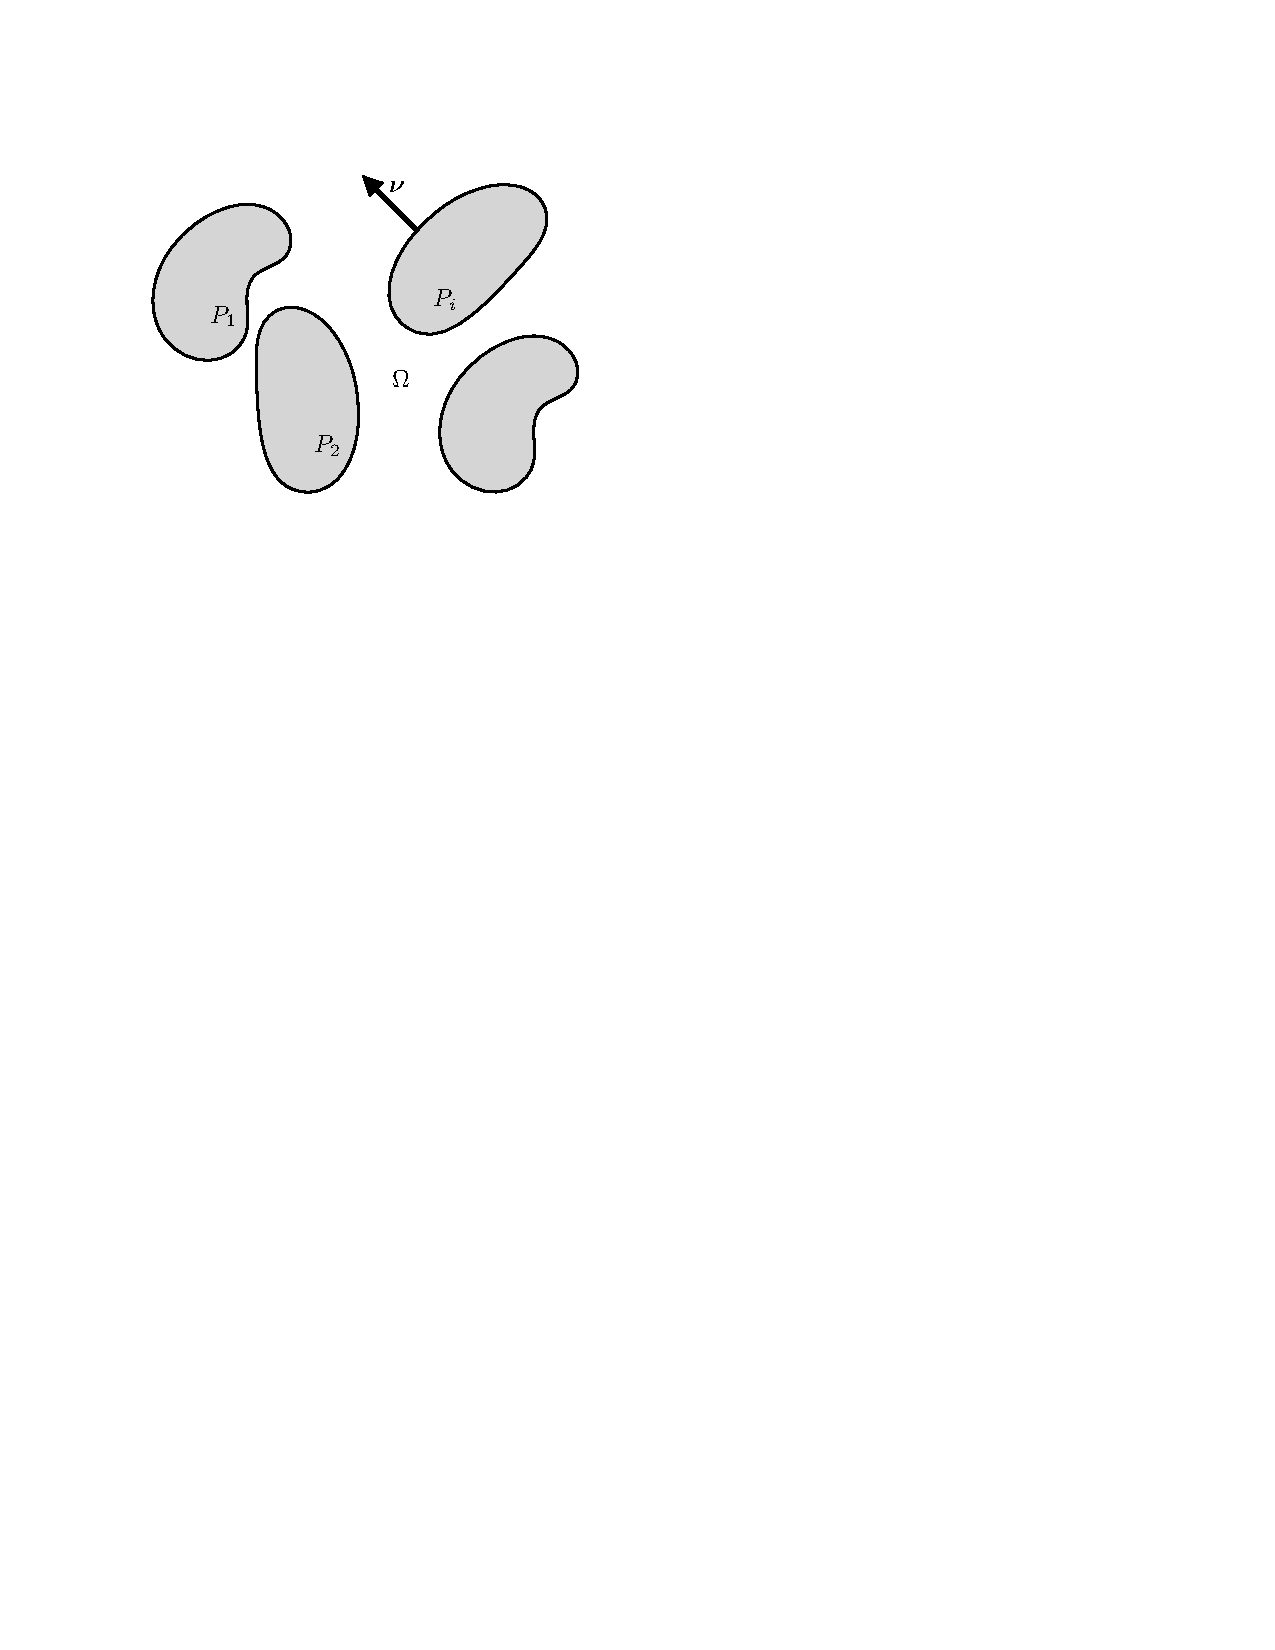
\includegraphics[width=0.23\textwidth]{figures/BG_fig1.pdf}}
\caption{ \footnotesize
A collection of rigid particles: $P_1,$ $P_2,$ $P_3, \ldots$. The
exterior domain $\Omega$ represents the solvent.}
  \label{fig:domain}
\end{wrapfigure}
\subsection{Hydrophobic Attraction Potential (HAP)}
\label{sec:HAP}
%Based on the physical origin of hydrophobicity,  we have devised a
%functional, called the hydrophobic attraction potential (HAP), to model
%hydrophobic forces~\cite{Fu2018_SIAM}. 
The motivation for the HAP concept stemmed from PI RR's work concerning
energy barriers in membrane
fusion~\cite{RyKlYaCo16,Chetal16}. By applying a mathematical, squared-gradient
theory for hydrophobic attraction between planar
surfaces~\cite{Eriksson1989,Lum1999,Menshikov2017,Marcelja1977}, PI RR
and collaborators resolved the long-standing issue of accounting for the
energy of a monolayer fissure surface during topological transitions.
Based on PI RR and YNY's coarse-grained membrane modeling
work~\cite{Fu2017}, the investigators devised a gradient theory for
arbitrary collections of hydrophobic and
amphiphilic particles. As a new method, HAP eliminates the costly calculation
of water by treating the solvent implicitly, is capable of representing
biologically-relevant morphologies, and avoids complicated
re-meshing schemes of continuum approaches by utilizing a particle-based
representation.

To define HAP, consider a collection of particles suspended in a
solvent. The region $\Omega \subset \mathbb{R}^3$ models the solvent
phase (Figure \ref{fig:domain}).
%The HAP must be an energy of the shape of the region because hydrophobic
%attraction is non-additive.
The boundary of the region is the union of water-particle interfaces
with unit normal $\boldsymbol{\nu}$. Some parts of this interface are
hydrophobic while others are hydrophilic. Hydrophobic interfaces disturb
the hydrogen bond structure of water~\cite{Luzar1987, Jonsson2006,
Varilly2011} and this disturbance comes with an energetic penalty that
is proportional to interfacial area. There is an additional decay
length, due to rapid fluctuation in the hydrogen bond network,
describing how far the restructuring extends into bulk water.

The above considerations motivate the following definition for HAP:
\begin{align}
\label{HAP}
  \Phi = \gamma \int_{\Omega} \rho |\nabla u|^2 + \rho^{-1}u^2 \,\dif V. 
\end{align}
The integrand contains
the decay length $\rho$
and a dimensionless scalar function $u(\mathbf{x})$ called the water activity.
The integrand has units of an inverse length, so
the volume integral has units of area. Multiplication by interfacial tension
$\gamma$ makes $\Phi$ an energy. 

To establish an attraction between interfaces, the water activity is not
arbitrary but rather is the solution of the screened Laplace
equation boundary value problem 
\begin{equation}
  \label{SL}
  -\rho^2 \Delta u + u = 0, \mbox{ } \mathbf{x} \in \Omega, \qquad
  u = f,  \mbox{ } \mathbf{x} \in \partial \Omega, \qquad 
  u(\mathbf{x}) \to 0, \mbox{ as } |\mathbf{x}| \to \infty.
\end{equation}
The boundary values $f$ define the degree of hydrophobicity of the
water-particle interface: $f=1$ describes a hydrophobic interface, and
$f=0$ describes a hydrophilic interface. Thus, $f$ encodes information
about the particles, and the parameters $\rho$ and $\gamma$ encode
information about the quality of the solvent~\cite{Israelachvili1954,
Discher2002}.
In the figures throughout the proposal, red is for $u = 1$ and blue is for $u = 0$.
In practice, we integrate~\eqref{HAP} by parts and
use~\eqref{SL} to obtain
\begin{equation}
\label{eq:HAP_easy}
\Phi = -\gamma \int_{\partial \Omega} \rho u \nabla u \cdot \boldsymbol{\nu} \,\dif S,
\end{equation}
thereby avoiding volume integral calculations.

The equations~\eqref{HAP} and~\eqref{SL} possess a number of
mathematical properties that mirror the phenomenological characteristics
of hydrophobic attraction. Specifically, solutions of~\eqref{SL} yield
an attractive force between hydrophobic bodies separated by water, and
this attraction decreases exponentially with the distance of
separation~\cite{Eriksson1989}. Using boundary layer analysis, the HAP
converges to a surface energy in the zero-decay length
limit~\cite{Lee2018, Lin2015, Shibata2004}. Finally, we have
demonstrated that the forces derived from HAP theory are
non-additive~\cite{Meyer2006, Fu2018_SIAM}. 
%The hydrophobic force has been implicated in the directed folding of proteins, 
%adhesion between biological membranes, but it is still unanswered as to whether
%the hydrophobic force of the form (\ref{HAP}--\ref{SL}) exists between small molecules. 

%As a summary of its mathematical properties,  the hydrophobic force
%is a non-additive, exponentially decaying surface force 
%that possesses a separation of length scales. These properties suggest 
%a boundary value problem formulation of the hydrophobic force.  
%The non-additivity of the hydrophobic force has to do with the fact that there is no superposition
%principle for including subdomains in boundary value problems. 
%The exponential decay is a property of a second order elliptic partial differential equation (PDE). 
%Finally, the separation of scales come from boundary layers, 
%where the energy of the boundary layer in the zero-thickness limit corresponds to macroscopic interfacial tension.
%Overlapping boundary layers correspond to microscopic hydrophobic attraction, 
%and the boundary layer thickness corresponds to the decay length of attraction.
%
%
%\section{Previous Results by the PIs}
%\label{sec:results}
%
%%In our paper \cite{Fu2018_SIAM}, 
%PIs RR and YNY developed the HAP model (\ref{HAP}--\ref{SL})
%to quantify the macroscopic assembly and mechanics of a lipid bilayer membrane in solvents \cite{Fu2018_SIAM}.
%%We formulated the boundary value problem as a second-kind
%%integral equation (SKIE), presented in the Section (). 
%%The simulated fluid-particle systems exhibit a variety of multiscale behaviors over both time and length.
%%Over short time scales, the numerical results showed self-assembly for model lipid particles. 
%%For large system simulations, the particles formed realistic configurations like micelles and bilayers. 
%%Our collections showed that these amphiphilic particle bilayers  possessed mechanical properties of a 
%%lipid  bilayer  membrane  that  are  consistent  with other results in the literature.   
To define the particle dynamics, let $P_1$, $P_2$, \ldots, $P_N$ be a
finite collection of disjoint, rigid, and closed particles each with
a Lipschitz boundary. Assume that the label $f$ is an element of the
Sobolev space $H^1(\Omega)$. The functional~\eqref{HAP} has a minimizer
among all functions $u$ equaling $f$ on the boundary in the sense of
trace. Conversely, from maximum principles and energy estimates, the
solution of~\eqref{SL} is unique and minimizes~\eqref{HAP}. Taking the
first variation of~\eqref{HAP}, i.e.~the derivative with respect to the
domain~\cite{Bandle2015, Schiffer1954, Grinfeld2010}, yields a
symmetric, rank-two tensor called the hydrophobic stress (equation (2.3)
in~\cite{Fu2018_SIAM}):
\begin{align}
  \label{stress}
\boldsymbol{\sigma}_{\text{hydro}} = \gamma \rho^{-1} u^2 I + 2\rho
  \gamma \left(\frac{1}{2}|\nabla u|^2I - \nabla u \nabla u^T\right).
\end{align}
%
%To obtain \eqref{stress}, we observe that the potential $\Phi$ is a function of the particle position and orientations.
%This is because the particle configuration defines the shape of $\Omega$ and the boundary data $f.$ 
%Taking the derivative of \eqref{HAP} with respect to particle configurations, and using the boundary value problem \eqref{SL}
%in a critical way leads to the surface term \eqref{stress}.  
%
Integrating the hydrophobic stress over the surface of particle $P_i$
reveals the hydrophobic force, and torque on each particle 
\begin{align}
  \label{forceandtorque}
  \mathbf{F}_{\text{hydro},i} = \int_{\partial P_i} \boldsymbol{\sigma}_{\text{hydro}}
  \cdot \boldsymbol{\nu} \,\dif S,\quad
  \mathbf{G}_{\text{hydro},i} = \int_{\partial P_i} (\mathbf{x}-\mathbf{a}_i) \times
  (\boldsymbol{\sigma}_{\text{hydro}} \cdot \boldsymbol{\nu}) \,\dif S,
\end{align}
relative to the center of mass $\mathbf{a}_i$. This system is force- and
torque-free (\S\ref{subsec:specific_aim_2}). To avoid particle
collisions, we define an excluded volume potential $\Phi_{\text{repul}}$
that diverges whenever tubular neighborhoods of adjacent particles
overlap. The total potential, force, and torque are then
\begin{equation}
\label{eq:total_poten}
\Phi = \Phi_{\text{hydro}} + \Phi_{\text{repul}},\quad
\mathbf{F}_{i} = \mathbf{F}_{\text{hydro},i} + \mathbf{F}_{\text{repul},i},\quad
\mathbf{G}_{i} = \mathbf{G}_{\text{hydro},i} + \mathbf{G}_{\text{repul},i}.
\end{equation}

To supply viscous dissipation, we incorporate the mobility problem
flow for a rigid body suspension in Stokes flow:
\begin{equation}
\label{eq:stokes}
\begin{aligned}
  &-\mu \Delta \mathbf{u} + \nabla p = 0, \quad \mathbf{x} \in \Omega, \qquad 
  \nabla \cdot \mathbf{u} = 0,  \quad \mathbf{x} \in \Omega,\\
  &{\bf u}(\mathbf{x}) \to 0 \quad \text{as}\ |\mathbf{x}|\to \infty,\qquad 
  \mathbf{u}(\mathbf{x})|_{\partial P_i} = \mathbf{v}_i +
\boldsymbol{\omega}_i\times(\mathbf{x} - \mathbf{a}_i),\\
&\int_{\partial P_i}\boldsymbol{\sigma}\cdot {\bf n} \dif S=-{\bf F}_i, \quad
\int_{\partial P_i} (\mathbf{x} - \mathbf{a}_i)\times (\boldsymbol{\sigma} \cdot \mathbf{n}) \dif S =-{\bf G}_i.
\end{aligned}
\end{equation}
Here, $\mu$ is the fluid viscosity; the first two equations state that
the fluid motion is a divergence-free Stokes flow; the third equation
specifies that the fluid velocity vanishes at infinity; the fourth
equation enforces a rigid body motion on each particle, where
$\mathbf{v}_i$ and $\boldsymbol{\omega}_i$ are unknown translation and
angular velocities; and the last two equations state that the net
viscous forces and torques with fluid shear stress $\boldsymbol{\sigma}$
balance \eqref{eq:total_poten}.


The time integration of particle configurations goes as follows:
\textbf{(i)} solve the BVP~\eqref{SL} for the screened Laplace equation,
\textbf{(ii)} determine the rigid body forces and
torques~\eqref{forceandtorque}, \textbf{(iii)} solve the Stokes mobility
problem~\eqref{eq:stokes} for the rigid body motions, and \textbf{(iv)}
update the particle configuration.  Numerical challenges and how these
challenges are overcome are described in \S\ref{subsec:specific_aim_2}.

%%(2YY: 
%We have intentionally ignored  latency in the variational 
%calculations. At issue is that any change in the particle position involves the relaxation time 
%of the hydrogen bond network. To remedy this, we could parametrize a path for the 
%particles configuration as a function of physical time. Then the rate of change
%of hydrophobic interaction includes the surface hydrophobic stress as calculated, but also a body term 
%for time change of activity, assuming we model hydrogen bond relaxation by diffusion. 
%The diffusion time, however, is extremely small since hydrogen bond lifetimes are on the order 
%of $10^{-11}$ s \cite{Israelachvili1954}. This setup is analogous  to that of a Kelvin-Voigt material,
%where viscoelastic deformations exponentially approach the purely elastic deformation.  
%%)

\begin{wrapfigure}[14]{l}{0.35\textwidth}
\centerline{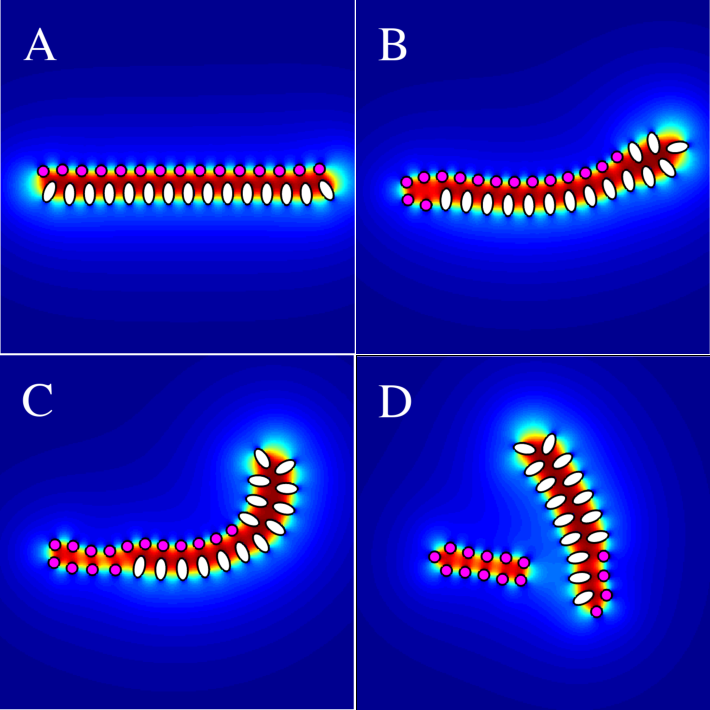
\includegraphics[width=0.34\textwidth]{figures/PW_fig2.pdf}}
  \vspace{-8pt}
  \caption{\label{fig:demixing} \footnotesize An initial assembly of
  small and large particles spontaneously segregates into two smaller
  bodies.}
\end{wrapfigure}
The HAP formulation is, to our knowledge, the first demonstration of
bilayer self-assembly by a continuum-based interaction
model~\cite{Noguchi2001, Farago2003, Brannigan2006, Brooks2009,
Wang2013}. Our simulations use Janus particles to model lipid
amphiphiles which are popular in material science and physics for
creating functional materials~\cite{Lee2014, Lee2013}. Janus particles
are typically spherical with a biphasic material label on either
hemisphere, endowing the particle with
a directional order. We model an
elongated lipid by elliptical particles with the hydrophobic label
defined along the ellipse's axis. 
Under the hydrophobic force, with
excluded volume, the Janus particles spontaneously merge and realign
to form bilayers. This occurs only as a result of energy minimization
and does not require artificial inputs.
%

%
It is worth emphasizing that the HAP model uses only a few parameters:
interfacial tension, decay length, repulsion strength, and particle
shape. For example, an elastic modulus for stretching a vesicle from
micropipette manipulation calibrates our interfacial tension
parameter. This is in direct contrast with pair-potential-based
approaches in MD simulations and coarse-grained models where many more
parameters are required~\cite{Varilly2011, Wang2013}.
%MD simulators have also made measurements and lately there is better and better agreement with reality. 
%But even the simplest coarse grained models based on pair potentials for lipids has many more parameters \cite{Varilly2011,Wang2013} . 

%As a proof of concept, our work has already tested for elastic energies
%for bending, stretching, and tilt of the bilayer assembly. The elastic
%coefficients derived from the HAP simulations show strikingly positive
%agreement with experimentally determined values~\cite{Fu2018_SIAM}.
%Encouraged by these results and the hydrodynamic simulations of
%bilayer assembly, the PIs propose to extend the HAP model to make direct
%comparisons with experimental results \S\ref{subsec:specific_aim_1} and to
%establish that the HAP model has the capability to model
%flow phenomena across length scales and time scales
%\S\ref{subsec:specific_aim_2} using efficient, high-order numerical
%methods \S\ref{subsec:specific_aim_3}.

%\begin{wrapfigure}[14]{l}{0.35\textwidth}
%\centerline{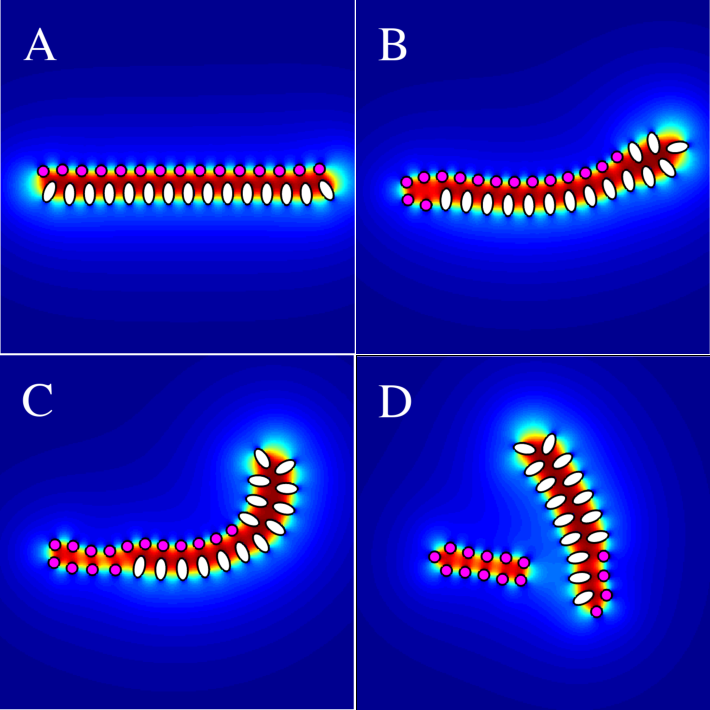
\includegraphics[width=0.35\textwidth]{figures/PW_fig2.pdf}}
%  \vspace{-8pt}
%  \caption{\label{fig:demixing} \footnotesize An initial assembly of
%  small and large particles spontaneously segregates into two smaller
%  bodies.}
%\end{wrapfigure}
Over the past decades, researchers have used a number of mathematical
tools to simulate vesicles in a shear flow, including lattice
Boltzmann~\cite{KaouiHartingMisbah2011_PRE}, coarse-grained Brownian
dynamics~\cite{NoguchiTakasu2002_BJ}, phase
field~\cite{DuLiuWang2004_JCP,BibenKassnerMisbah2005_PRE}, level
set~\cite{DoyeuxGuyotChabannesEtAl2013_JCAM}, boundary
integral~\cite{Shravan09,Rahimian15}, and immersed boundary
approaches~\cite{KimLai2010_JCP,KimLai2012_PRE,HuLaiSeolEtAl2016_JCP}.
Most of these approaches assume a mathematical surface, whether
implicitly or explicitly, and define an elastic bending energy of the
surface. These vesicle studies built off of numerical methods for
calculating energy minimizing steady equilibrium shapes of lipid bilayer
membranes, vesicles, and red blood cells. These approaches range from
the finite element~\cite{Bartels,Peng13,RyKlYaCo16,Sinha15},
phase field~\cite{Du05,QiangDu08,Lowengrub13}, and immersed
boundary methods~\cite{Hu,Hu13, KimLai2010_JCP}. PI RR and collaborators
led in part the development of phase field functionals of membrane
elastic energy and approaches to coupling membrane elasticity to
fluids~\cite{0951-7715-18-3-016,Du05,DuEuler,QiangDu09}.


%The vesicle obeys fluid
%transport and in turn the fluid balances shear stress with the vesicle's bending force. 

Our HAP approach differs from these prior methods in a number of
respects. First, we do not assume a surface. Rather, we 
assume a collection of amphiphilic particles. The
collection of amphiphiles minimize hydrophobic interactions by
sequestering hydrophobic tails in the form of a bilayer, and the
particles' excess free energy gives rise to an elastic bilayer energy.
The second difference lies in the fluid-interface coupling. Here, the
associated mobility problem~\eqref{eq:stokes} is more complicated than
dealing with a stress boundary condition or diffusive surface force
because the fluid velocities are for individual rigid body motions at each
particle surfaces. Finally, the HAP model directly addresses the
existence of multiple phases. We can vary lipid length, spontaneous
curvature, and bending rigidity by introducing different particle shapes
and hydrophobic boundary conditions (Figure~\ref{fig:demixing}). In
contrast, continuum theory deals with multiple phases through additional
surface densities that must satisfy specialized transport
equations~\cite{Lowengrub07, MikuckiZhou17}. 


\begin{wrapfigure}[6]{r}{0.35\textwidth}
\centerline{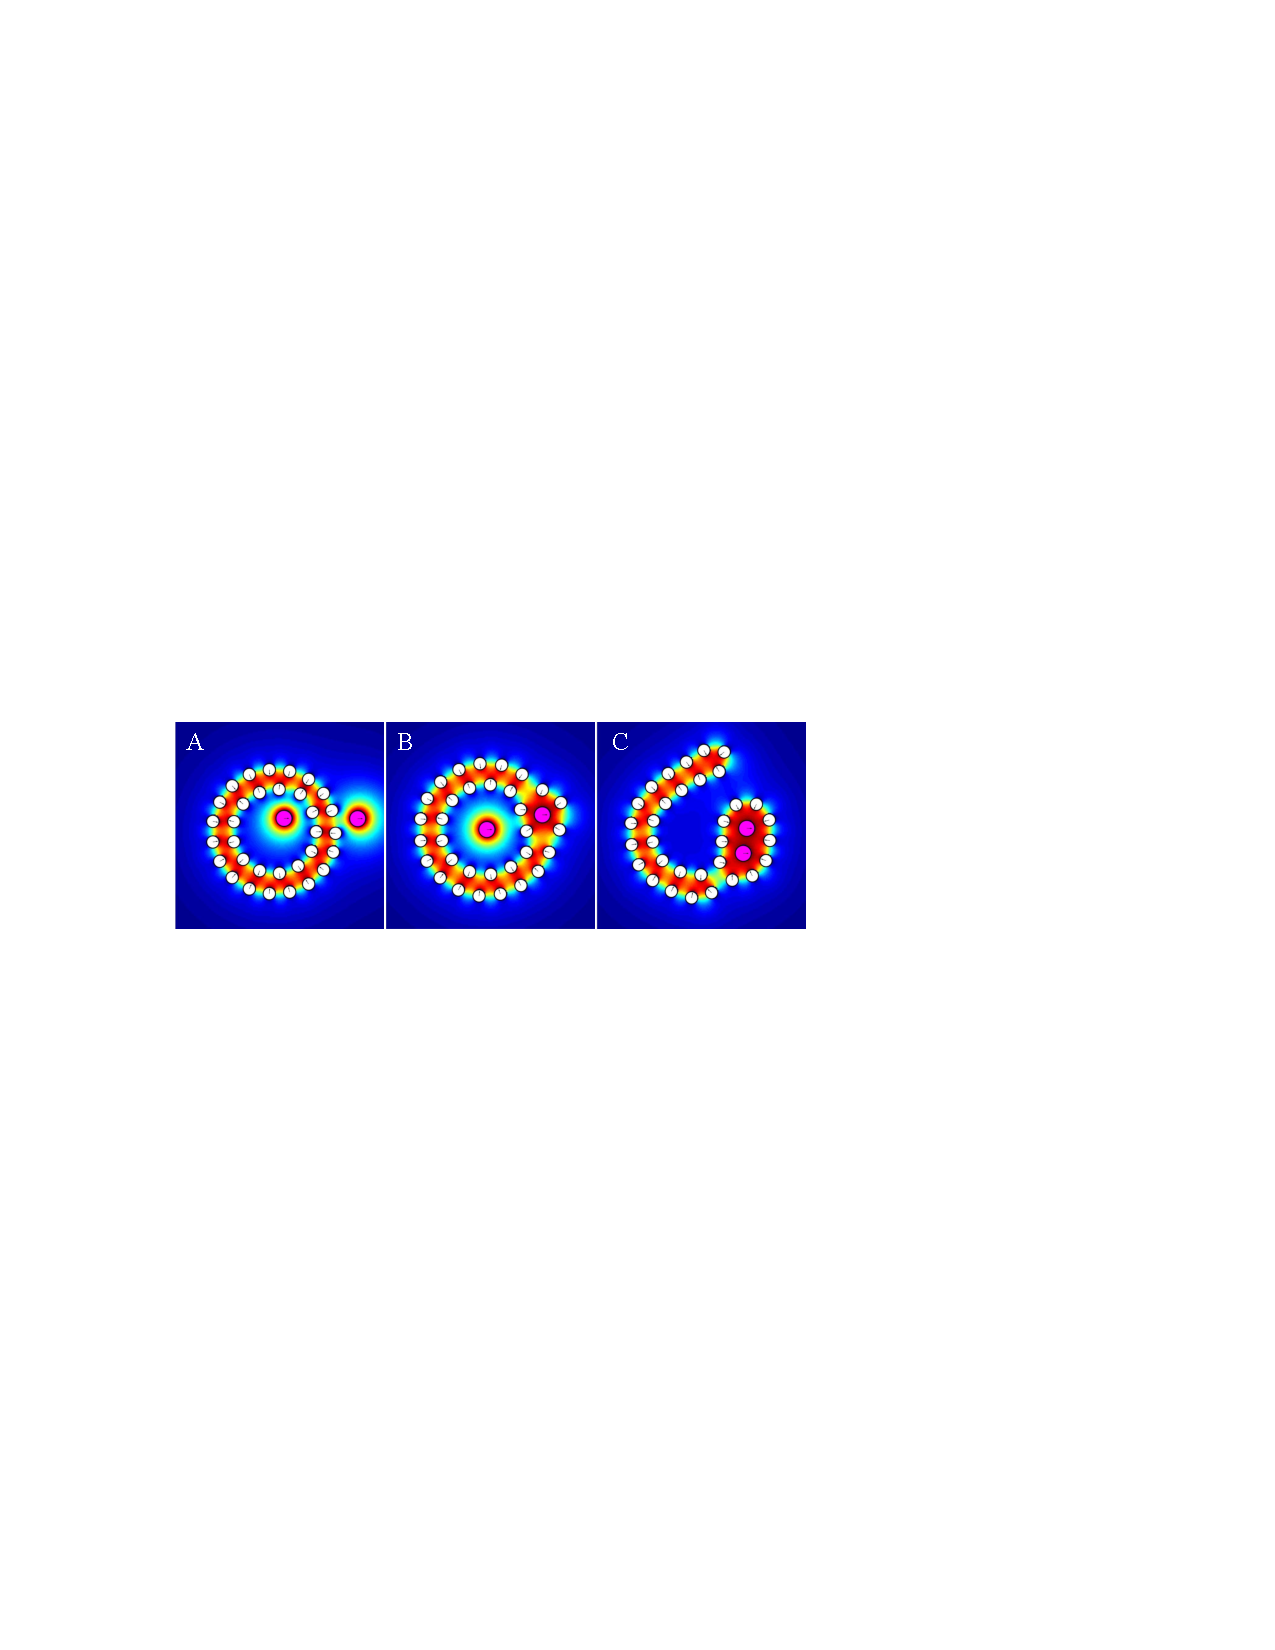
\includegraphics[width=0.34\textwidth]{figures/Lysis.pdf}}
  \vspace{-8pt}
  \caption{\label{fig:lysis} \footnotesize Two hydrophobic particles
  enter and then lyse the circular bilayer.}
\end{wrapfigure}
The greatest strength of using the HAP to model a lipid bilayer membrane is
the ability to form discontinuities (interfacial singularities) from first
physical principles without any artificial manipulation to rearrange the
interface (Figures~\ref{fig:demixing} and~\ref{fig:lysis}). For
example, using the HAP model to simulate a vesicle under a shear flow
that is strong enough to cause the vesicle membrane to rupture (see
\S\ref{sec:preliminary_work}), we expect the HAP model to capture the
reorganization of lipid molecules on the scales of membrane thickness
($\sim 5$ nm), which is a nearly impossible task using phase-field or
immersed boundary methods without extreme refinement around the membrane
and artificial treatment of reconnection during the topological change
of an interface \cite{doi:10.1063/5.0009734, LiAn-Chang16,
doi:10.1098/rspa.2012.0505, doi:10.1137/130941432, Feetzl18,
doi:10.1137/16M1108406}.

%Some disadvantages are that the hydrophobic interaction does not constrain vesicle volume. 
%Instead, changes in volume are rate limited by inter-particle spacing,
%which may be undesirable in case of a mathematically strict volume constraint.
%% set vesicle volume, as is done in the study of liposomes
%%using auxiliary constraint equations for instance. 
%%Also, the boundary integral method formulation
%%relies on linearity of the Stokes equations. There has been some progress in
%%boundary integral methods for the non-linear Navier-Stokes equations [ref].
%%We point out that some non-Newtonian effects in polymers are a consequence of hydrophobic
%%and steric molecular interactions like the ones presented in this proposal. 





%
%
%The next few years provide the ideal window of opportunity for demonstrating the physical realism 
%of the HAP model. 
%
%
%
%The definitions and calculations for fully three-dimensional bilayer elastic energies are described in greater
%detail in Specific Aim 1. 
%


% 4.1 pN / nm = 4.1 pN nm / nm^2 = 4.1(1e-12)(1e-9) N m/(1e-18) m^2 = 4.1 (1e-3) J/m^2 = 4 mJ/m^2 
% pN/nm = mJ / m^2 and 1 kT / nm = 4 mJ / m^2 so stretching 40 gives 40  
% erg / cm^2 =  (1e-7) J/(1e-4) m^2 =   1e-3 J/m^2 =  mJ/m^2  
% 120 mJ / m^2 
% 10 erg / cm^2 = 10 pN nm / nm^2 = 2 kT / nm^2 
%

%\section{Proposed Research}
%\label{sec:proposed-work}
%The goal of the proposed research is to develop fast,
%high-order-accurate, parallel numerical algorithms for large-scale
%simulations of the collective hydrodynamics of janus particles in a solvent in both two- and three-dimensions.
%First we summarize some basic formulation and preliminary results
%\cite{Fu2018_SIAM} in \S~\ref{subsec:bie} and \S~\ref{subsec:3dbie}.
%We then describe outstanding numerical issues that we propose to address  in \S~\ref{subsec:proposed_research}.

%\section{Proposed Research}
%\label{sec:proposed-work}
%The goal of the proposed research is to develop fast,
%high-order-accurate, parallel numerical algorithms for large-scale
%simulations of the collective hydrodynamics of  amphiphilic particles in a viscous solvent.
%%
%Based on the integral formulation in \S~\ref{subsec:bie} and \S~\ref{subsec:3dbie}, we have demonstrated that 
%our potential theory approach can efficiently simulate self-assembly of 
%amphiphilic particles into two-dimensional micelles, bilayer membranes,
%and vesicles \cite{Fu2018_SIAM}.
%%
%While these results show great potentials in simulating the collective hydrodynamics of amphiphilic particles and
%reproducing mechanical properties of their bilayer assembly, 
%several outstanding issues need to be addressed for such approach to be efficiently applied to three-dimensional 
%collective hydrodynamics of amphiphilic particles.
%
%the two-dimensional hydrodynamics of amphiphilic particles 
%
%the two-dimensional results in \cite{Fu2018_SIAM} are in agreement with the 
%
%
%First we summarize some basic formulation and preliminary results
%\cite{Fu2018_SIAM} in \S~\ref{subsec:bie} and \S~\ref{subsec:3dbie}.
%We then describe outstanding numerical issues that we propose to address  in \S~\ref{subsec:proposed_research}.
% -----------------------------------------------------------------------------
%\subsection{Proposed research: High-order discretization of surface integrals in three dimensions}\label{subsec:proposed_research}
%% -----------------------------------------------------------------------------
%% {{{
%The practical application of integral equation methods requires the
%accurate evaluation of boundary integrals with singular, weakly
%singular or nearly singular kernels.  Historically, these issues have
%been handled either by low-order product integration rules (computed
%semi-analytically), by local modifications of a smooth
%rule~(e.g.~\cite{alpert,kapur,sidi}), by singularity
%subtraction/cancellation (e.g.~\cite{duffy,bruno1,bruno2,davis_1984,graglia_2008,hackbusch_sauter_1994, jarvenpaa_2003,khayat_2005,kress_boundary_1991,schwab_1992, ying_2006}), by kernel
%regularization and asymptotic analysis (e.g.~\cite{beale1,beale2,goodman_1990, haroldson_1998, lowengrub_1993,schwab_1992}), or by the
%construction of special purpose ``generalized Gaussian'' quadrature
%rules (e.g.~\cite{ggq1,ggq2,ggq3}).
%In the complex analytic case, additional methods
%have been developed by \citet{helsing_2008a} for off-surface
%evaluation. It should be noted that in the two-dimensional case,
%several of these alternatives provide extremely effective schemes,
%especially the kernel-splitting method developed by Johan Helsing
%\cite{helsing_integral_2009,helsing_tutorial_2012,helsing_2008a} since
%they all permit local adaptivity and high order accuracy.
%
%The high-order quadrature rules for the evaluation of surface integrals
%in three dimensions are much less developed than the line integrals in two
%dimensions. For example, there are no Gaussian quadratures for integraing
%polynomials on a flat triangle, even though efficient quadratures
%\cite{xiao2010cma,vioreanu2014} have been
%developed recently for such purpose. For weakly singular or singular integrals,
%\cite{bremer2012jcp,bremer2013jcp} constructed high-order quadratures
%for surface integrals on a general triangle, while \cite{gimbutas2013sisc}
%presented a fast algorithm for integrating $1/r$-type singular integrals
%for surfaces that are homeomorphic to a sphere. We would like to propose
%to study the so-called quadrature by expansion (QBX) scheme~\cite{klockner2013jcp,qbx2}
%for the evaluation
%of both singular and near-singular surface integrals encountered in the
%discretization of BIEs in three dimensions. Conceptually, the idea of the QBX
%to evaluate singular, hypersingular and near singular integrals
%on smooth surfaces is more or less straightforward. That is, the surface is discretized
%into smooth triangles and smooth high-order quadratures are applied to evaluate
%the expansion coefficients
%on all source triangles with the QBX expansion center placed at a point off the surface.
%One may then form a suitable expansion (for example, a Taylor expansion) around that
%center and evaluate this expansion back at the target point on the surface (or close
%to the surface in the near singular case). Compared to the competing aforementioned
%quadrature schemes, the QBX quadrature is attractive
%because it offers a clear path for being extended to: \textbf{(1)}
%handle any ambient and source dimensionality, \textbf{(2)} integrate
%any kernel, and thereby be usable for a very large range of PDEs and
%boundary conditions, \textbf{(3)} handle any singularity, including
%hypersingular operators, \textbf{(4)} be usable with any high-order surface
%discretization, \textbf{(5)} generate well-conditioned discrete
%operators to which iterative methods such as GMRES~\cite{gmres} can be
%applied in a black-box fashion, \textbf{(6)} be computationally
%efficient enough to be applied on the fly (without the need to store
%quadrature tables), \textbf{(7)} integrate well with fast algorithms
%such as the Fast Multipole Method. 
%
%In practice, there are still many issues that need to be resolved.
%For example, there are now many variants of QBX including global and local
%QBX~\cite{klockner2013jcp,rachh2017jcp}, the target-specific QBX~\cite{siegel2018jcp},
%kernel-independent QBX~\cite{abtin2018bit}, and
%quadrature by two expansions~\cite{ding2019arxiv}. The coupling of the QBX
%and the FMM may also lead to certain instability issues which may require
%some changes in the fast multipole method~\cite{wala2018jcp}. Similar
%to other quadrature methods, there have been an extensive study on the QBX
%methods in two dimensions, while its three dimension
%version~\cite{wala2019jcp,af2018sisc,siegel2018jcp,wala2019arxiv} has not been
%fully studied and the implementation is even more scarce. We plan to investigate
%the accuracy and the convergence order of the various QBX schemes mentioned above,
%its coupling with the FMM, parallel implementation issues for large-scale
%problems, and the application to our target problems.



